\documentclass[12pt]{book}
\usepackage{graphicx}
\usepackage{subfig} % make it possible to include more than one captioned figure/table in a single float
\usepackage[utf8]{inputenc}
\usepackage{hyperref}
\usepackage[intlimits]{amsmath}
\usepackage{amssymb}
\usepackage{tkz-euclide}
\usepackage{tikz}
\setlength{\oddsidemargin}{15.5pt} 
\setlength{\evensidemargin}{15.5pt}
\pretolerance=2000
\tolerance=3000
\renewcommand{\figurename}{Figura}
\renewcommand{\chaptername}{Cap\'{i}tulo}
\renewcommand{\contentsname}{\'{I}ndice}
\renewcommand{\tablename}{Tabla}
\renewcommand{\bibname}{Bibliograf\'{i}a}
\renewcommand{\appendixname}{Ap\'endices}

\title{Colisión de 2 galaxias elipticas con M1/M2 = 3, head-on}
\begin{document}

\section*{Pasos}
\begin{enumerate}


\item Construimos varios modelos de galaxias elipticas con halo y sin halo para ver el efecto del halo.
Para construir los  modelos iniciales se usaron: 
\begin{itemize}
\item Modelo de Hernquist para el halo
$\Phi(r) = \frac{-GM}{r + a}, a = scale length, r_J = (1 + sqrt(2))*a $ \\

\item El modelo de Jaffe para el bulbo
$\Phi(r) = \frac{-G M }{r_J}  ln(\frac{r} {r + r_J})$\\
\end{itemize}
donde
\begin{itemize}
\item M = total mass 
\item rJ = half mass radius
\item Al transformar a unidades adimensionales G=M=1
\end{itemize}
los 2 modelos obtenidos:
\begin{itemize}
\item Esinhalo.xvp solo bulbo 20000 particulas con masa  4.99999987E-05
\item Econhalo.xvp bulbo(10000 particlas con masa 9.99999975E-06) y halo(40000 particulas con masa 2.24999985E-05)
\end{itemize}

Miramos los 2 modelos con nora y vemos que la masa total es 1 en los 2 asi que no hace falta escalarlos

\item Relajar el modelo \\
Siempre hay que ejecutar tree500 para relajar los modelos iniciales
aunque esté en equilibrio virial(Ep = -2Ec) para usar el mismo epsilon(softening)\\
Parametros modificados en TEEEPAR:
\begin{itemize}
\item tCross = sqrt(R**3/M), R = radio media masa(lo miramos con nora), M = 0.5(el modelo ya esta en unidades adimensionales)
\item dt = tCross / 10
\item totalTime = 20(-30) * tCross
\item si elegimos totalTime = 20 * tCross entonces nsteps = 200 siempre
\item eps = 0.125(-0.2) * RadioMediaMasa
\end{itemize}


\item ejecutar kepler para sacar los parametros para setorb\\
Despues de relajar los modelos miramos el radio total calculamos  la separación de los 2 objetos  sep = 3*Rt y la introducimos en kepler después de escoger la opción 2.
Se obtienen Vr, Vt(en el caso de una órbita  parabólica: eccentricity = 1 Vt = 0, pero para eccentricity=0.7 - órbita elíptica Vt>0) y Period(el tiempo necesario para el encuentro)

\item ejecutar setorb con la entrada sep y velocidad obtenidas de kepler y salida el modelo con los 2 objetos en orbita
\item escalar el modelo obtenido: M2/M1 = 1/1.33 = 0.751, R2/R1 = sqrt(M2/M1) = 0.8671
\item ejecutar tree500 con el modelo obtenido con setorb dejando los demas parámetros igual que en el paso, sólo modificamos nsteps con el valor un poco mas grande que el Period obtenido en kepler. El valor sale demasiado grande y es inválido asi que ejecuto tree500 varias veces con el nsteps = 2000


\end{enumerate}
\section*{Análisis}
\begin{itemize}
\item Como he ejcutado tree500 varias veces y no he guardado TREELOG, TREEORB y TREEAM intermedios, estos ficheros se sobreescriben cada vez que se ejecuta tree500. Hay que sacar los valores del modelo de otra forma
\item numberModel que aparecerá en los gráficos es el número de modelo: la relacion con el tiempo es t = noutbod * numberModel * dt, donde noutbod(20) y dt son los parámetros de TREEPAR, entonces totalNumberModels = nsteps / noutbod
\item Los valores del radio para fracciones de masa de 0.1, 0.5, 0.8, 0.99 se obtuvieron con un script python que ejecutó Rm para todos los modelos (200/20 = 10 modelos)


\begin{figure}[!h]
 \centering
 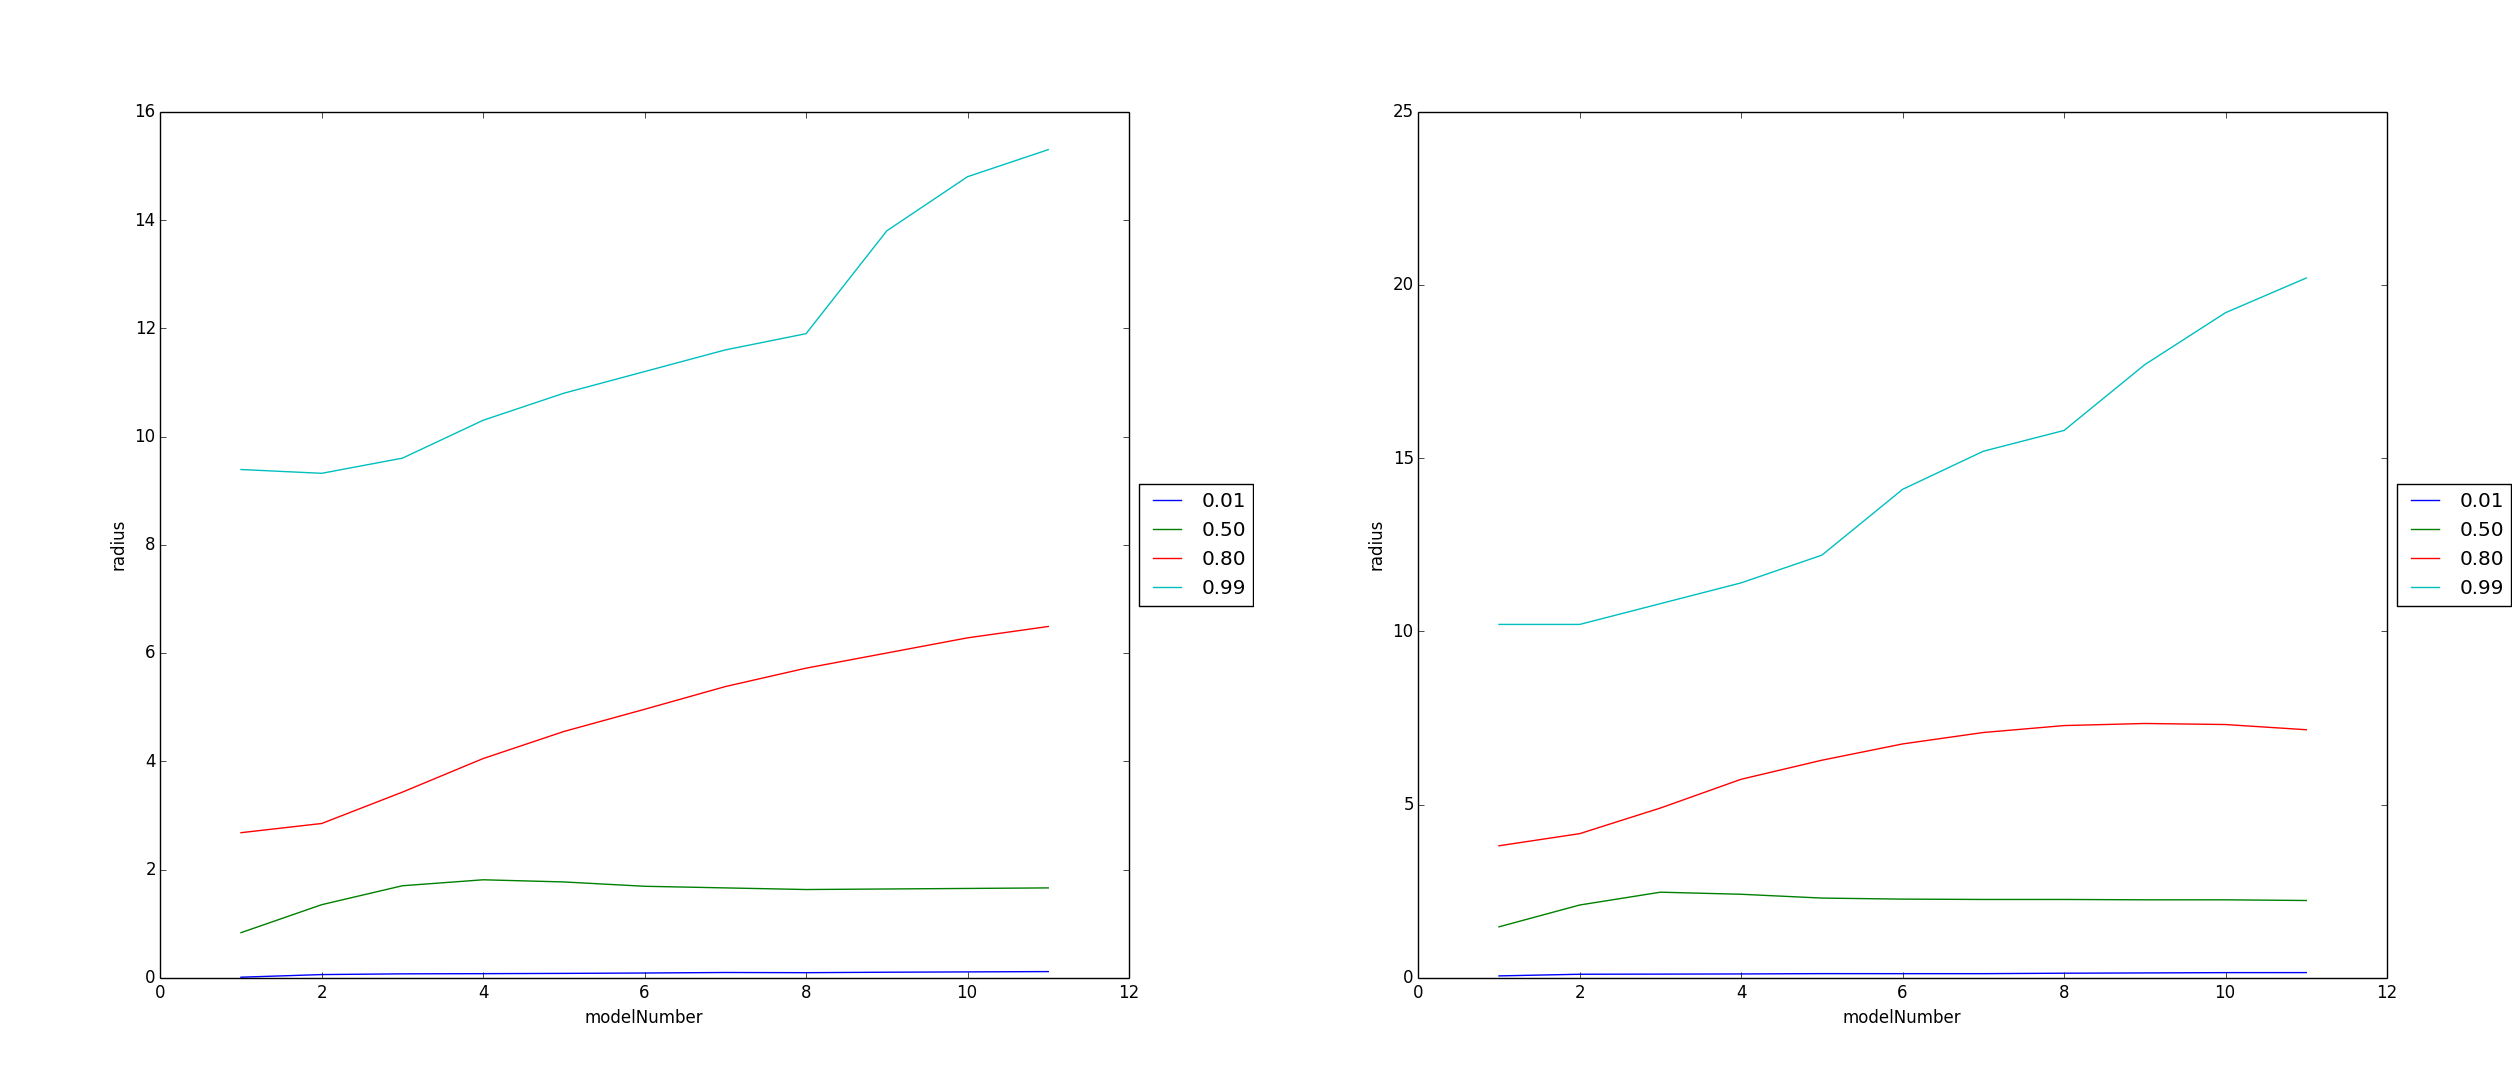
\includegraphics[scale=0.2]{imgRad1.png}
 \caption{\emph{Relajación del modelo(primera ejecucion de tree500), a la izquierda el modelo sin halo, a la derecha el modelo con halo\\
	donde se representa el valor del radio correspondiente a varias fracciones de masa(ver la leyenda)
}}
 \label{Fig: 1}
\end{figure}

\item las 2 con halo\\
con halo numberModels = 265  $\implies$ Time = 1335.6 menor que period (calculado con kepler) 4171.98
Representamos el radio del sistema binario con la evolucion(ahora el radio para la fraccion 1 esta bien)


\begin{figure}[!h]
 \centering
 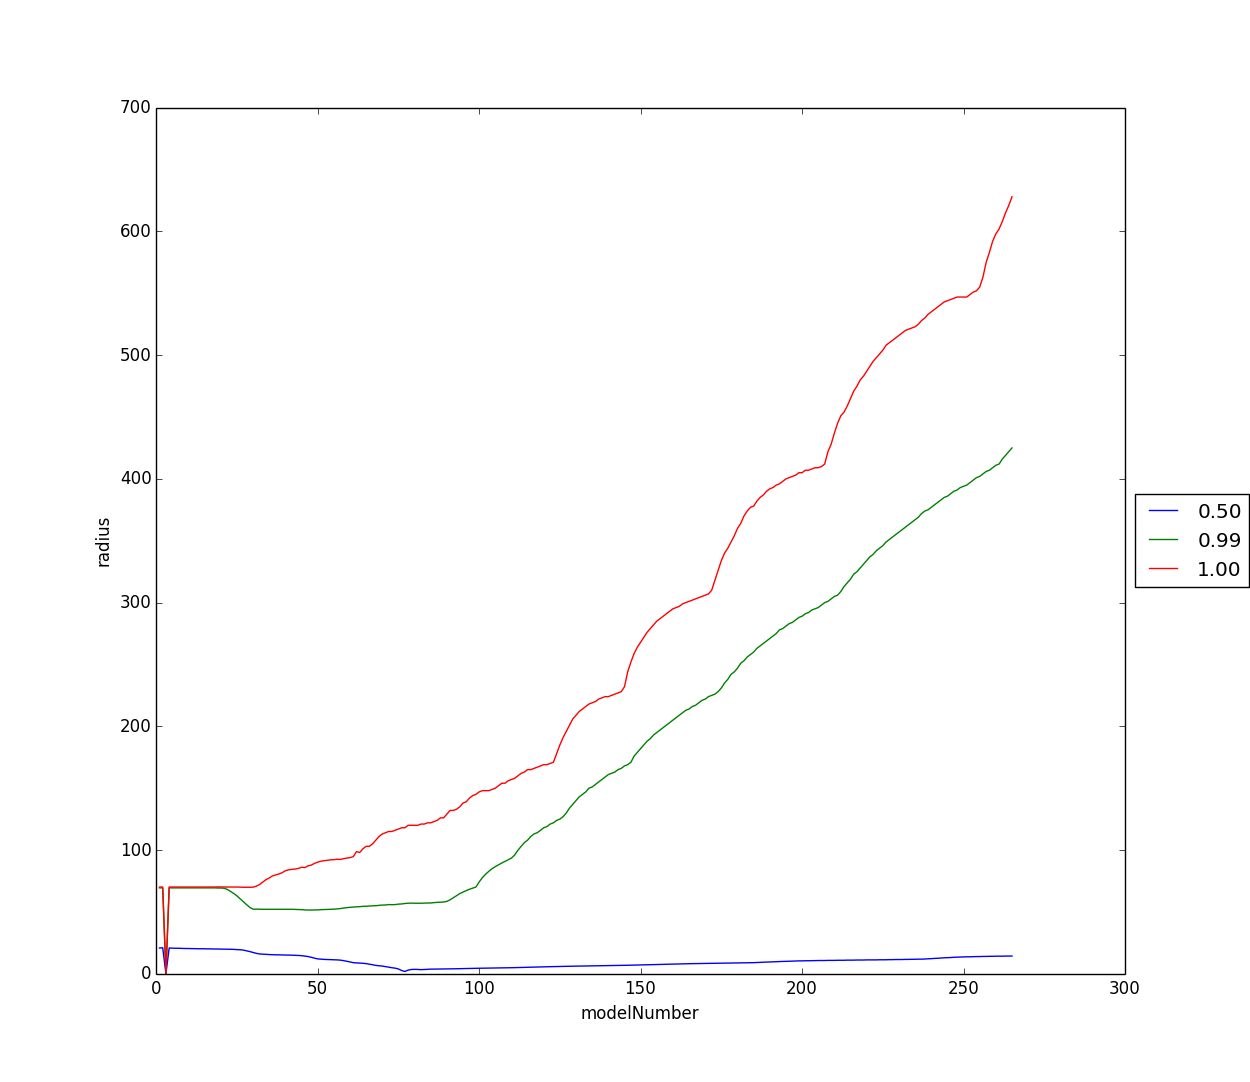
\includegraphics[scale=0.4]{imgRadcon2.png}
 \caption{\emph{}}
 \label{Fig: 2}
\end{figure}

Distancia entre los centros (de masa) de las 2 galaxias
Se obtuvo ejecutando para cada model (script python que usa expect con nora)
\begin{verbatim}
bodsrange 1 fin1
medcent
bodsrange fin1+1 fin2
medcent
\end{verbatim}
donde fin1 es es numero de la ultima particula del primer sistema (en este caso 50000) y fin2 es el numero total de particulas
La distancia entre los 2 centros está definida por la salida del segundo medcent 
median position :    1.801E-04   1.954E-01  -8.183E-02
en este caso la distancia es  (1.801E-04 **2 +  1.954E-01**2+  8.183E-02**2)**0.5 = 0.2118427278336691



\begin{figure}[!h]
 \centering
 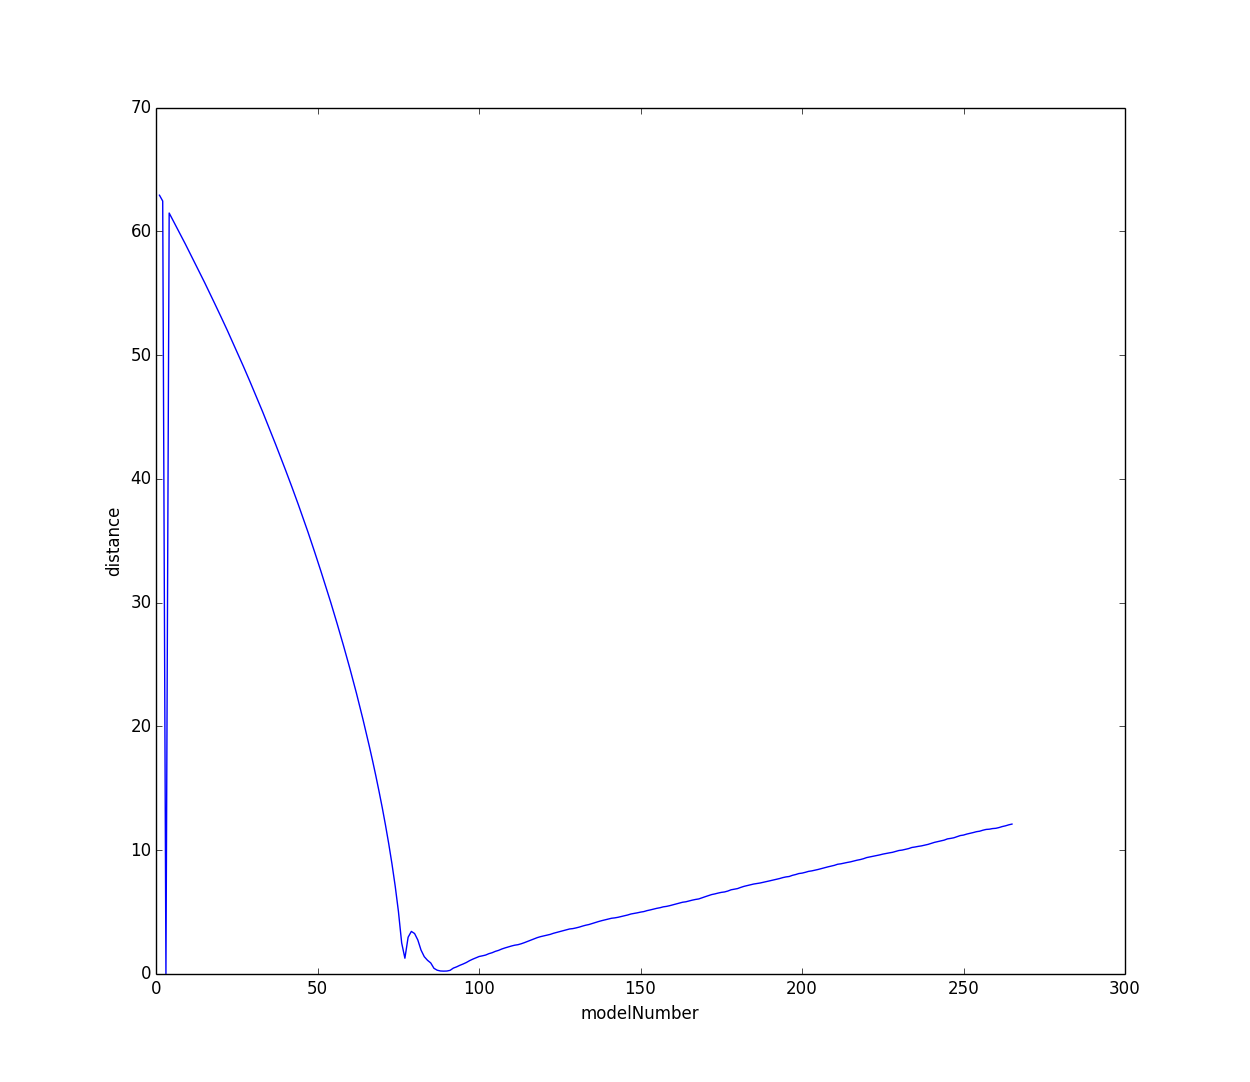
\includegraphics[scale=0.4]{imgDistcon.png}
 \caption{\emph{Distancia entre los centros de las 2 galaxias obtenida en nora con medcent}}
 \label{Fig: 3}
\end{figure}

Como se ve en el radio del sistema binario igual que en la distancia de los 2 centros para el modelNumber 3 hay una caída en el gráfico y mirando el modelo 3 con nora la imagen obtenida para el radio max 10 (points 10) es un punto(PORQUE?)

\begin{figure}[!h]
 \centering
 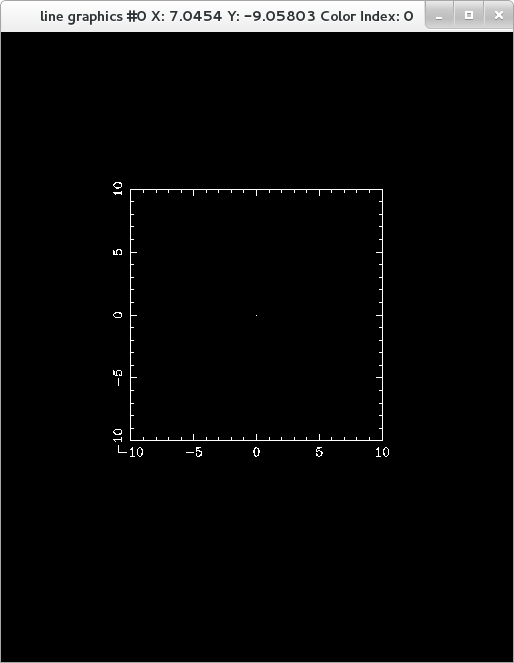
\includegraphics[scale=0.5]{imgConModel3Points10.png}
 \caption{\emph{points 10 para modelo 3}}
 \label{Fig: 4}
\end{figure}

El siguiente  mínimo para la distancia es para el modelo 89(con el valor mínimo de la distancia 0.2118427 comprobado en nora) y la imagen para radio 50 (points 50) es la siguiente:

\begin{figure}[!h]
 \centering
 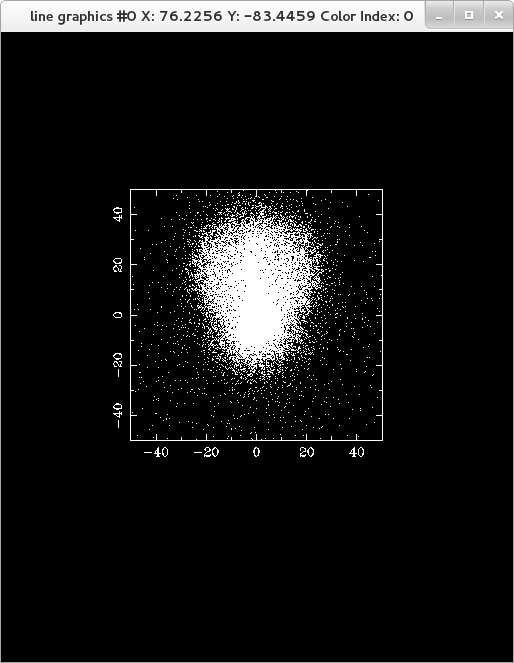
\includegraphics[scale=0.5]{imgConModel89Points50.png}
 \caption{\emph{points 50 para modelo 89}}
 \label{Fig: 5}
\end{figure}

medcent centra por la mediana de posiciones, para centrar por el centro de masas hay que usar cmcent
El radio y la distancia entre los centros de los 2 sistemas se pueden obtener tambien directamente del modelo(sin usar nora), para ello sacamos los modelos para cada modelNumber con xvp-asc lo que hay que hacer si queremos representar como varía la velocidad(en nuestro caso nos interesa la velocidad radial) o el momento angular en el tiempo

Calculando el centro de masas de cada sistema con :
$\sum{m_ir_i}$ (M=1), donde $m_i$ es la masa de cada particula y $r_i$ es la posición 
y luego haciendo la diferencia entre los 2 valores se obtiene el gráfico para la distancia(el gráfico es diferente del gráfico obtenido con medcent pero es muy parecido al gráfico obtenido en nora con cmcent - tienen el mismo mínimo para modelNumber = 77)

\begin{figure}[!h]
 \centering
 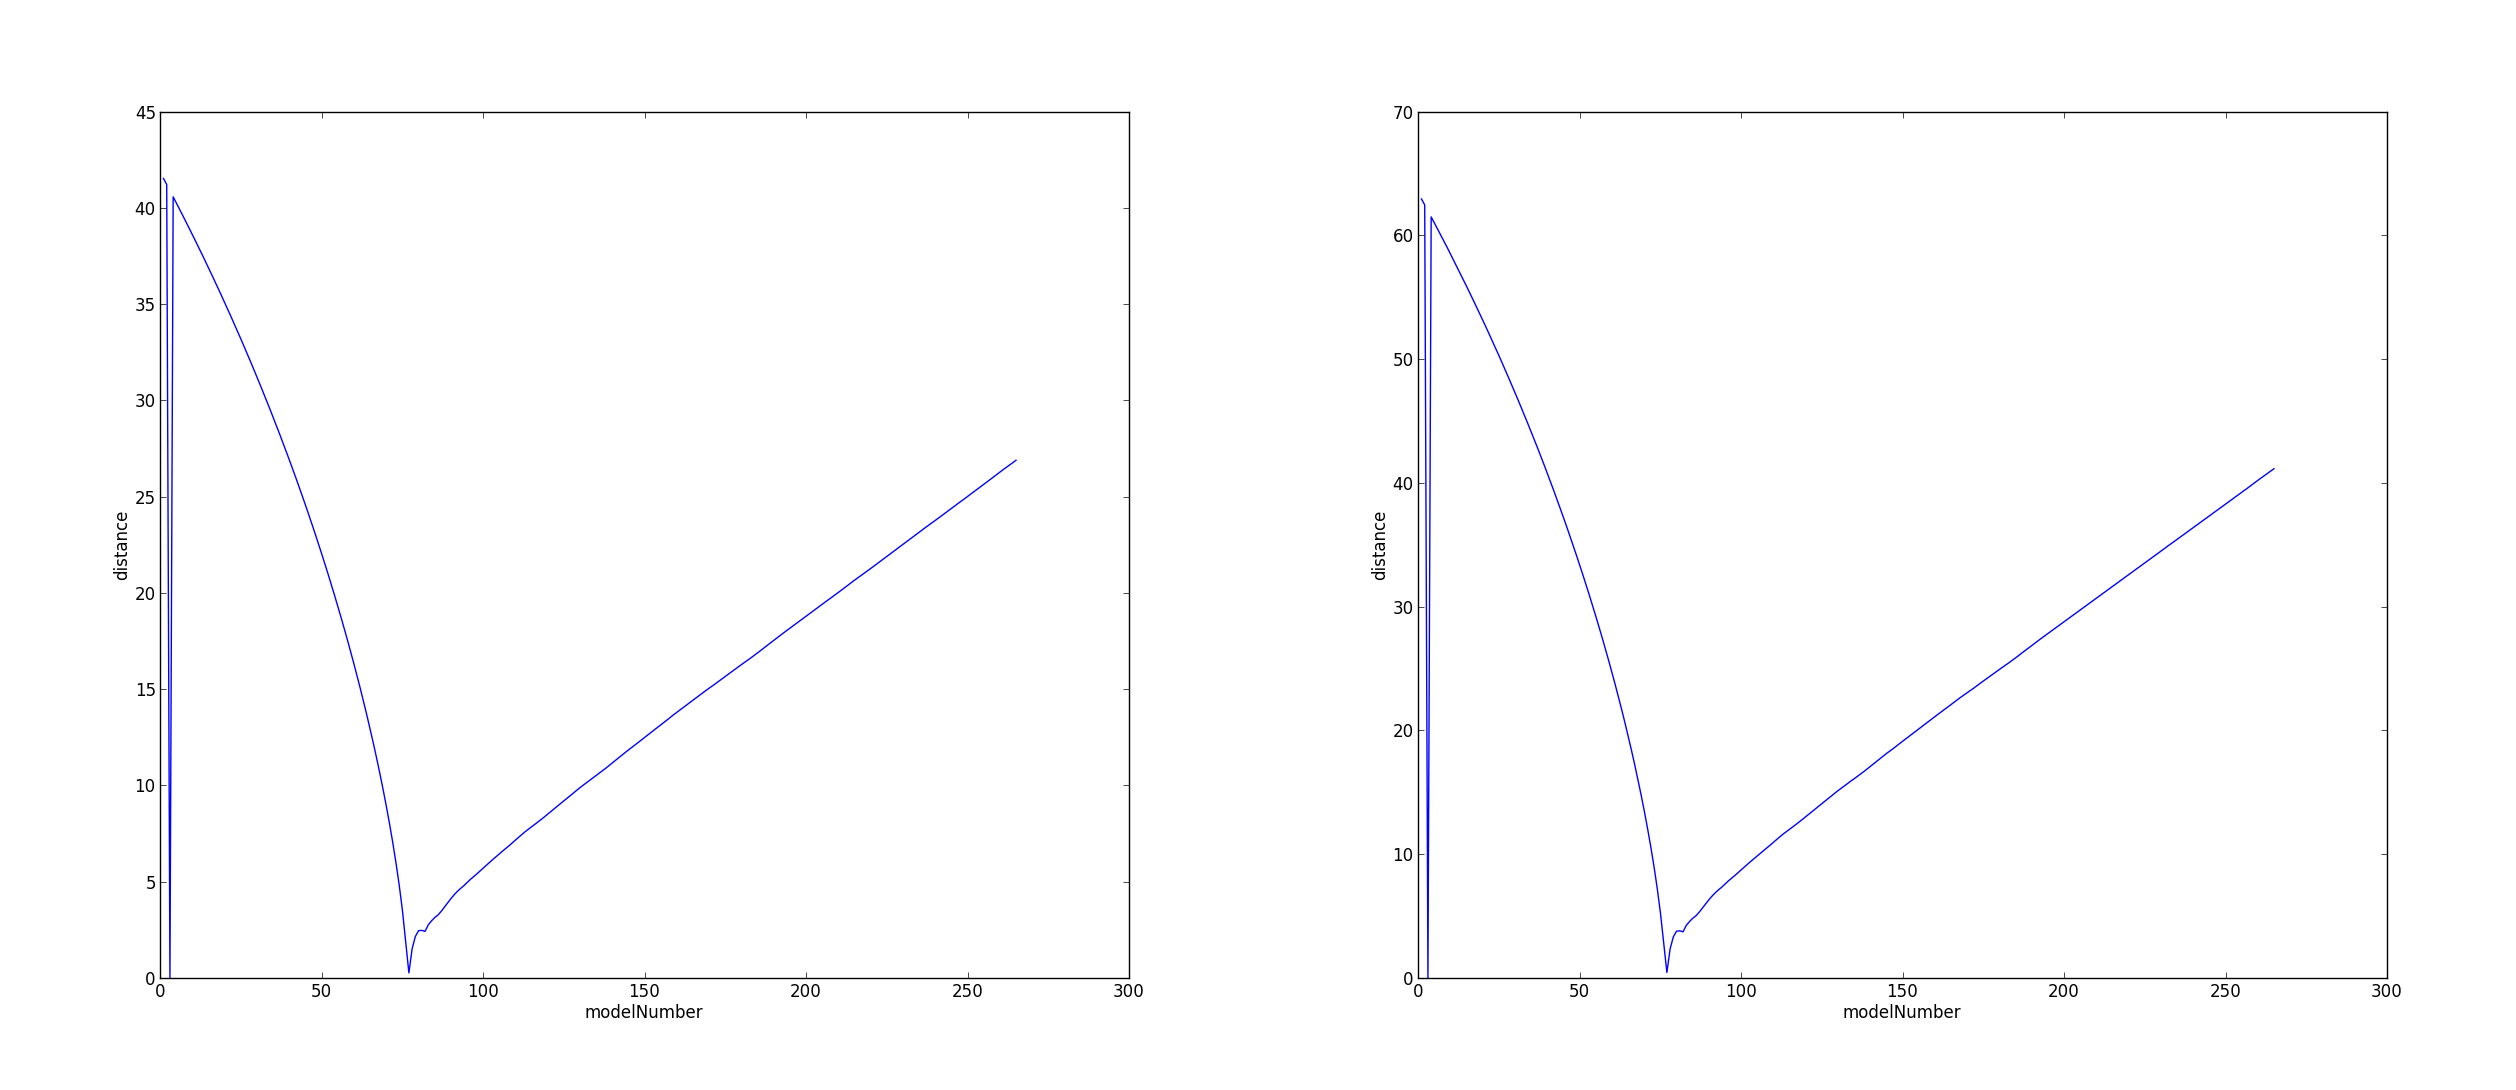
\includegraphics[scale=0.2]{imgDistcon2Comb.png}
 \caption{\emph{La evolución de la distancia de los centros de masa de las 2 galaxias: a la izquierda calculado con cmcent y a la derecha calculada de los valores del modelo}}
 \label{Fig: 5}
\end{figure}
\end{itemize}

El mínimo en el modelo 3 sigue igual(el problema del modelo anterior), pero el siguiente mínimo es esta vez 77 y la imagen obtenida con nora al radio máximo 50 es:

\begin{figure}[!h]
 \centering
 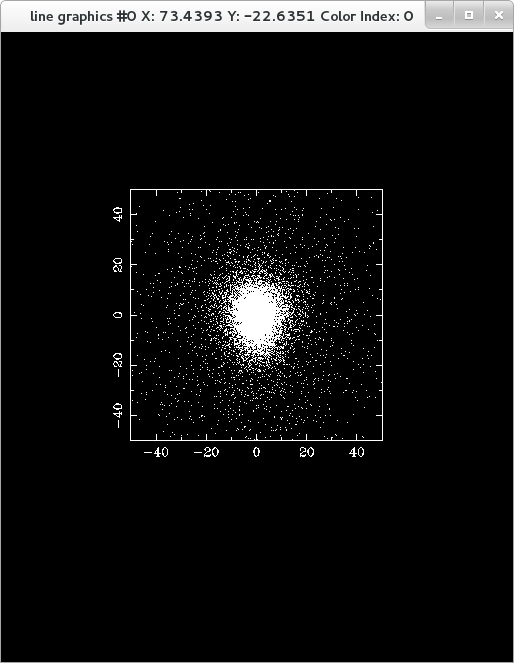
\includegraphics[scale=0.5]{imgConModel77Points50.png}
 \caption{\emph{points 50 para modelo 77}}
 \label{Fig: 5}
\end{figure}
\end{document}

